\documentclass[onecolumn,12pt]{article}

\usepackage{amssymb}%Blacksquare
\usepackage[margin=0.7in]{geometry}
\usepackage{amsmath,parskip,graphicx} 
\usepackage[utf8]{inputenc} %not clear effect
\usepackage[T1]{fontenc} %not clear effect
\usepackage[english]{babel}% not clear effect
\usepackage{float} %used for fixed tables with [H]
\usepackage{amsthm}
\usepackage{textcomp}
\usepackage{enumerate}
\usepackage{wrapfig}
\usepackage{cite}
\usepackage{amssymb}
\usepackage{epstopdf}
\usepackage{inputenc}
\usepackage{array}
\usepackage{booktabs}
\usepackage{subfig}
\usepackage[justification=centering]{caption}
\usepackage{array}% http://ctan.org/pkg/array	
\usepackage[nottoc]{tocbibind}
\usepackage{fancyhdr} %doing header and footer
\usepackage{tikz} %initializing the package
\usetikzlibrary{calc}
\usepackage{listings}


\restylefloat{table}
\numberwithin{equation}{section}

\title{University Physics Competition - 2016}
\author{The spheric triangle}
\date{\today}   

\pagestyle{fancy}
\fancyhf{}
\lhead{Reactor Waste Disposal}
\chead{University Physics Competition}
\rhead{Team 351}
\rfoot{Page \thepage}

\renewenvironment{abstract}{
\begin{center}
\begin{minipage}{0.85\textwidth}
\rule{\textwidth}{0pt}}
{\par\noindent\rule{\textwidth}{0pt}
\end{minipage} \end{center}}

\begin{document}

\begin{titlepage}
\begin{center}
\vspace{5mm}
\huge{Space Methods of Reactor Waste Disposal} \\
\vspace{5mm}
\Large{Team 351: Problem A - Reactor Waste Disposal} \\
\vspace{5mm}


\textbf{Abstract:}\\
\vspace{5mm}
\end{center}

\begin{abstract}

This paper investigates the possibility of sending reactor waste of mass $m_f - m_0$ into space using a spacecraft with empty mass $m_0 = 2 \cdot 10^6$ kg. The trajectories of the spacecraft carrying the payload were described by Hohnmann transfers, and the momenta changes were approximated using Tsiolkovsky rocket equations using a bipropellant liquid rocket with $u = 4.4000 \text{ }km/s$. First, a theoretical analysis of the trajectories based on Kepler`s and Newton`s laws was employed, yielding results for the required changes in velocity $\Delta v$ and fuel consumption $\Delta m$. Two different tactics were analysed: sending the spacecraft directly into the Sun, and into the Main Asteroid Belt. The first method proved very costly, as the amount of fuel required when hitting the Sun is $ \Delta m'_1(R_{S2} = 445.71 \text{ }m_f)$ and when the spacecraft evaporates in the corona of the Sun is $ \Delta m'_1(R_{S1} = 223.74 \text{ }m_f)$, but with a rather easy and quick implementation. An innovative solution is to send the rocket on a higher orbit such that the velocity becomes negligibly small and drop the waste towards the Sun, requiring at least $m'' = 15.373  \text{ }m_f$. Considering the Asteroid belt with its Kirkwood gaps, two radii $R_{A1} = 2.3250 \text{ }au$ and $R_{A2} = 2.8850 \text{ }au$ were targeted requiring fuel masses $\Delta m (R_{A1}) = 8.1518 \text{ }m_f$, $\Delta m (R_{A2}) = 12.316 \text{ }m_f$. This approach has the advantage of possible retrieval and of smaller costs. The Solar System was modelled using MatLab and the actual position and velocity of the planets were used, then the spacecraft was inserted in key positions, serving different purposes. All the theoretical obtained values were confirmed by the simulations, and the stability of the orbit in the asteroid belt was proven for simulations done. The safety of the storage is however depending on the asteroids collisions which cannot be predicted. It was concluded that storing the waste in the asteroid field is the easiest option and shows a longevity higher than $1000$ years.

\end{abstract}
\end{titlepage}
\newpage

\section{Introduction and Theory}

This paper attempts to shed light on the details and requirements, as well as reliabilities and dangers of two methods of reactor waste disposal into space. The first one is transferring the waste into a stable orbit within the main asteroid belt, and the other one is dumping it directly into the Sun. For this purpose, the following theoretical model was defined.

\subsection{Hohmann Transfer Orbit}
 The Hohmann Transfer Orbit$^{\text{\cite{hohmann1}}}$ represents an elliptical orbit used to transfer an orbiting spacecraft from one circular orbit of radius $R$ to another of radius $R'$. The transfer is achieved using two instantaneous engine impulses, one to move the spacecraft into the elliptical orbit with semi-major axis $(R+R')/2$, and one given at the apoapsis to lift the periapsis. If $R'>R$ both impulses are co-oriented with the velocity of the spacecraft as in fig. \ref{hohmann_pic}, and if $R'<R$ the impulses are oriented in the opposite direction of the satellite`s movement. For the proof, the case $R'>R$ is considered$^{\text{\cite{hohmann2}}}$. Suppose a small spacecraft of mass $m$ is orbiting with velocity $v$ a much larger body of mass $M$. The energy of the spacecraft can then be written as the sum of kinetic and potential energies as follows:
\begin{equation}
    H= T + V = \frac{1}{2}mv^2 - G \frac{mM}{R}
\end{equation}
Here $G= 6.67408 \cdot 10^{-11}$ $m^3 kg^{-1} s^{-2}$ denotes the gravitational constant. Newton's second law states that:
\begin{equation}
    F_G=G\frac{Mm}{R^2} = m \frac{v^2}{R_1}= F_{cf}
\end{equation}
Which allows us to write the velocity $v_1$ of the circular orbit with radius $R_1$ as:
\begin{equation}
    v = \sqrt{\frac{GM}{R}}
    \label{v1}
\end{equation}
The spacecraft then executes a thrust in the direction of its velocity, increasing its velocity by $\Delta v$. It then moves on an elliptical orbit until the distance to the massive body becomes $R'$, at which point it has velocity $v_t$. Conservation of angular momentum yields:
\begin{equation}
      (v + \Delta v)\cdot R = v_t\cdot R
      \label{mc}
\end{equation}

\begin{figure}[H]
\centering
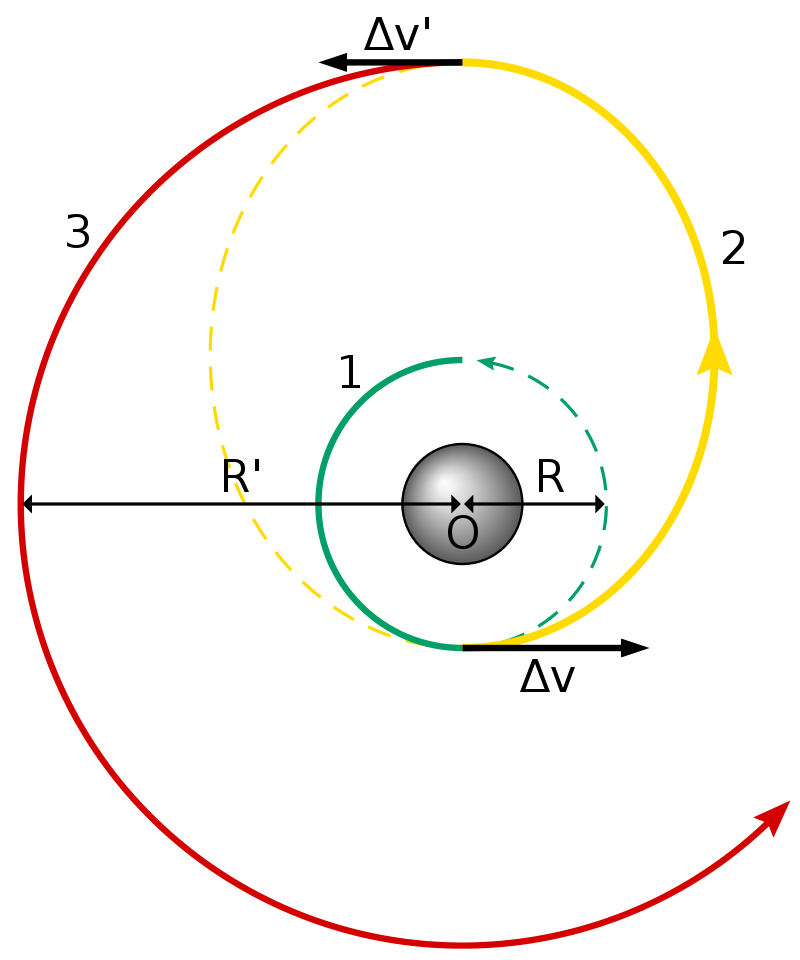
\includegraphics[width=0.8\linewidth]{figures/hohmann_transfer.png}
\captionof{figure}{Hohmann Transfer diagram from $R$ to $R'$ for the case $R'>R$ $^{\text{\cite{hohmann3}}}$}
\label{hohmann_pic}
\end{figure}

The total energy is conserved on the elliptical orbit, meaning that:
\begin{equation}
    \frac{1}{2}(mv+\Delta v)^2 - G \frac{mM}{R} = \frac{1}{2}mv'^2 - G \frac{mM}{R'}
    \label{ec}
\end{equation}
It then commits another thrust in the direction of its velocity, increasing it by an additional $\Delta v'$ such that its velocity becomes $v'$ (the velocity required for it to move on a circular orbit of radius $R'$), which is related to $R'$ similarly to (\ref{v1}):
\begin{equation}
    v' = \sqrt{G\frac{M}{R'}}
    \label{v2}
\end{equation}
The relation between $v_t$, $v'$ and $\Delta v'$ is therefore:
\begin{equation}
    v' = v_t + \Delta v'
    \label{v}
\end{equation}
Solving the obtained system of equations (\ref{v1}), (\ref{mc}), (\ref{ec}), (\ref{v2}) and (\ref{v}) yields for $\Delta v$ and $\Delta v'$:
\begin{equation}
    \Delta v = \sqrt\frac{GM}{R}\left( \sqrt\frac{2R'}{R+R'}-1\right)
    \label{theory1}
\end{equation}
\begin{equation}
    \Delta v' = \sqrt\frac{GM}{R'}\left( 1-\sqrt\frac{2R}{R+R'}\right) 
\end{equation}
Using a similar approach in the case $R'<R$ one would obtain the velocity changes $v_-$ and $v'_-$, oriented in the opposite direction :
\begin{equation}
    \Delta v_- = \sqrt\frac{GM}{R}\left(1 - \sqrt\frac{2R'}{R_1+R'}\right) 
    \label{hohmanntransfer}
\end{equation}
\begin{equation}
    \Delta v'_- = \sqrt\frac{GM}{R'}\left(\sqrt\frac{2R}{R_1+R'}-1\right) 
\end{equation}
The transfer time is given by, according to Kepler's third law and considering that the major semiaxis of the described ellipse is given by $a = (R_1+R_2)/2$:
\begin{equation}
    t_{transfer} = \sqrt{\frac{\pi^2(R_1+R_2)^3}{8GM}}
    \label{time}
\end{equation}

\subsection{Tsiolkovsky Rocket Equation}
The Tsiolkovsky rocket equation characterizes the motion of a spacecraft which thrusts itself by expelling part of its mass in the opposite direction, according to the conservation of momentum. Suppose the initial mass of the spacecraft is $m$, its velocity is $v$, and it uniformly exhausts an amount of mass $-\Delta m$ ($\Delta m$ represents the change in mass and thus has a negative value) in time $\Delta t$ with speed $u$ relative to itself. The conservation of momentum before and after the exhaust process yields:
\begin{equation}
    mv = (m + \Delta m)(v + \Delta v) -\Delta m(v - u)
    \label{momentum}
\end{equation}
Taking the limit of small $\Delta t$, $\Delta m$ and $\Delta t$ become differentials, meaning that equation (\ref{momentum}) becomes:
\begin{equation}
    mv = (m + dm)(v + dv) -dm(v - u)
\end{equation}
Considering that the resulting term $dm \cdot dv$ is the product of two differentials and is negligibly small, the equation above can be rewritten as:
\begin{equation}
    m dv = -u dm
\end{equation}
Rearanging the obtained equation and integrating using suitable limits yields:
\begin{equation}
    \int_{v_0}^{v} \frac{dv}{u}= -\int_{m_0}^{m} \frac{dm}{m}
\end{equation}
Solving the integrals and defining $\Delta v = v - v_0$ one obtains:
\begin{equation}
    \Delta v = u \ln \frac{m_0}{m}
    \label{tsiolkovsky}
\end{equation}

\section{Theoretical Analysis}

A simplistic model was investigated to gain some initial insight and numerical values. The starting point for this model represents the spacecraft carrying the waste orbiting the Sun in Earth's orbit ($R_E = 150.52 \cdot10^6 \text{ km}$). It is assumed that the spacecraft is already in a distant orbit around Earth, beyond Earth's sphere of gravitational influence, allowing Earth's pull to be neglected in the upcoming calculations. The Hohmann transfer orbit is then used to change the orbit of the spacecraft, and the resulting velocity change is related to the required mass of fuel using the Tsiolkovsky rocket equation.

\subsection{Reaching the distant orbit}

The desired distance such that the Earth`s gravitational influence can be neglected is given by the so-called radius of the sphere of gravitational influence $r_{SOI}$:

\begin{equation}
     r_{SOI} \approx a \left( \frac{m}{M}\right)^{2/5}
     \label{rSOI}
\end{equation}

For Earth, $r_{SOI}=0.924 \cdot 10^6$ km. Different methods can be used to achieve this scenario, however, once the rocket is stable in this orbit, the previous events are common for all the subsequent trajectories. Therefore, to analyse the problem, it is sufficient to look at the trajectories when the rocket leaves the orbits either towards the asteroid belt, or towards the Sun.

\subsection{Asteroid Belt Case}
In order to investigate the launch of the spacecraft into the Asteroid Belt two final orbits are considered, $R_{A1} =  2.3250 \text{ }AU = 347.82 \cdot 10^6 \text{ }km$ and $R_{A2} = 2.8850 \text{ } AU = 431.60 \cdot 10^6 \text{ }km$, described in the previous part. For both cases, the analytical computations are identical. Therefore a general case $R_{final}=R_A$ is investigated, and the values $R_{A1}$ and $R_{A2}$ will be substituted in the final result. According to the Hohmann transfer principle, in order to increase the radius of the orbit from $R_E$ to $R_A$, the required increase in velocity $\Delta v_1$  is given by: 
\begin{equation}
    \Delta v_1 = \sqrt\frac{GM}{R_E}\left( \sqrt\frac{2R_A}{R_E+R_A}-1\right)
\end{equation}
Respectively, after reaching the required radius $R_A$, another increase in velocity $\Delta v_2$ is required:
\begin{equation}
    \Delta v_2 = \sqrt\frac{GM}{R_A}\left( 1-\sqrt\frac{2R_E}{R_E+R_A}\right) 
\end{equation}
Using the gravitational constant $G = 6.6741 \cdot 10^{-11} \text{ }m^3 kg^{-1} s^{-2}$ and the mass of the Sun $ M = 1.9886 \cdot 10^{30} \text{ } kg$ the following results are obtained for the two possible choices for $R_A$:
\begin{equation}
    \Delta v_1 (R_{A1}) =  5.3895 \text{ } km/s
\end{equation}
\begin{equation}
    \Delta v_2 (R_{A1}) = 4.3519 \text{ } km/s
\end{equation}

\begin{equation}
    \Delta v_1 (R_{A2}) =  6.4656 \text{ } km/s
\end{equation}
\begin{equation}
    \Delta v_2 (R_{A2}) = 4.9257 \text{ } km/s
\end{equation}
The total mass $m_i$ of the spacecraft before the two propulsions can be written as:
\begin{equation}
    m_i = m_f + \Delta m_1 + \Delta m_2
\end{equation}
Here $m_f$ represents the mass of the spacecraft after the two propulsions, $\Delta m_1$ denotes the amount of fuel exhausted during the first speed-up, and $\Delta m_2$ is the mass of fuel exhausted during the second one. Using the Tsiolkovsky rocket equation (\ref{tsiolkovsky}) for each propulsion, the required amounts of fuel can be related to the previously obtained velocity changes $\Delta v_1$ and $\Delta v_2$ as follows:
\begin{equation}
    \Delta m_1 = m_f e^{\Delta v_2/u} (e^{\Delta v_1/u}-1)
\end{equation}
\begin{equation}
    \Delta m_2 = m_f (e^{\Delta v_2/u}-1)
\end{equation}
Using the effective exhaust velocity $c = 4.4000 \text{ }km/s$ (typical value for a bipropellant liquid rocket) \cite{rocketengine} and the previously obtained values for $\Delta v_1$ and $\Delta v_2$ yields:
\begin{equation}
    \Delta m_1 (R_{A1}) = 6.4631 \cdot m_f
\end{equation}
\begin{equation}
    \Delta m_2 (R_{A1}) = 1.6887 \cdot m_f
\end{equation}

\begin{equation}
    \Delta m_1 (R_{A2}) = 10.252 \cdot m_f
\end{equation}
\begin{equation}
    \Delta m_2 (R_{A2}) = 2.0633 \cdot m_f
\end{equation}
Assuming that the spacecraft was only loaded with enough fuel to make the two speed-ups, the total amount of fuel required to bring the spacecraft to a stable orbit in the asteroid field is (in terms of the mass $m_f$ of the spacecraft with an "empty tank"):
\begin{equation}
    \Delta m (R_{A1}) = \Delta m_1 (R_{A1}) + \Delta m_2 (R_{A1}) = 8.1518 \cdot m_f
    \label{fma1}
\end{equation}
\begin{equation}
    \Delta m (R_{A2}) = \Delta m_1 (R_{A2}) + \Delta m_2 (R_{A2}) = 12.316 \cdot m_f
    \label{fma2}
\end{equation}
The transfer times for these cases are, according to (\ref{time}):
\begin{equation}
    t_{A1} = 1.074 \text{ years}
\end{equation}
\begin{equation}
    t_{A2} = 1.357 \text{ years}
\end{equation}

\subsection{Falling into the Sun}
In a scenario similar to the movie "Sunshine" (2007), when the Sun is dying and humanity sends a nuclear payload to "reignite" it, the first approach investigated in this section is the case when a thrust in the opposite direction is used, lowering the velocity of the spacecraft by $\Delta v'_1$. It will then "descend" towards the Sun using the Hohmann principle. However it is not necessary to hit the Sun, considering that the Sun's Corona is its hottest part, with temperatures reaching $10^6 \text{ } K$. Therefore, a final orbit radius $R_{S1} = 3.0000 \cdot 10^6 \text{ }km$ is sufficient to meet our requirements. If however one would insist on "hitting" the Sun, the final orbit radius the radius of the Sun would be taken: $R_{S2} = 6.9570 \cdot 10^5 km$. Similarly to the previous case, computations are made for the general case $R_{final} = R_S$, and the two investigated values for the final radius are substituted in the final result. Using the Hohmann propulsion principle for the "slow-down" thrust yields:
\begin{equation}
    \Delta v'_1 = \sqrt\frac{GM}{R_E}\left(1 - \sqrt\frac{2R_S}{R_E+R_S}\right) 
\end{equation}
The numerical result is then:
\begin{equation}
    \Delta v'_1 (R_{S1}) = 23.826 \text{ } km/s
\end{equation}
\begin{equation}
    \Delta v'_1 (R_{S2}) = 26.848 \text{ } km/s
\end{equation}
As the spacecraft gets to the aphelion of its Hohmann trajectory it is already in the Sun's Corona and evaporates due to the high temperature and radiation (in the case $R_S$ is taken to be $R_{S1}$) or hits the Sun (for $R_S = R_{S2}$). Since the spacecraft has in either case reached its destination, it is unnecessary to do an additional slow-down thrust.  Again, according to the Tsiolkovsky Rocket Equation (\ref{tsiolkovsky}) the required amount of fuel $\Delta m'_1$ is related to the velocity change $\Delta v'_1$ as follows:
\begin{equation}
    \Delta m'_1 = m_f (e^{\Delta v'_1/u}-1)
\end{equation}
Which yields a numerical result of:
\begin{equation}
    \Delta m'_1 (R_{S1}) = 223.74 m_f
    \label{gandon1}
\end{equation}
\begin{equation}
    \Delta m'_1 (R_{S2}) = 445.71 m_f
    \label{gandon2}
\end{equation}
The transfer times for these cases are, according to (\ref{time}):
\begin{equation}
    t_{S1} = 67.127 \text{ days}
\end{equation}
\begin{equation}
    t_{S2} = 65.622 \text{ days}
\end{equation}
The obtained results for $m'_1 (R_{S1})$ and $m'_1 (R_{S2})$ are more than one order of magnitude larger than the fuel masses $\Delta m (R_{A1})$ (\ref{fma1}) and $\Delta m (R_{A2})$ (\ref{fma2}) required to send the spacecraft into a stable orbit in the asteroid field. It can therefore be concluded that such an approach is downright inefficient. The high fuel consumption in this case is due to the necessity of canceling the initial angular momentum of the spacecraft. The only apparent advantage of sending the waste directly into the Sun is the fact that it takes about six times less than it would take for it to reach the asteroid field.

However there is another approach that can be taken in order to send the nuclear waste into the Sun. The spacecraft could be transferred to a more distant circular orbit on which its velocity is much lower using a similar approach to the one described in the previous case, and once the spacecraft enters this orbit a thrust can be used to completely stop the spacecraft. Once stopped, the spacecraft can release the nuclear waste which will fall without having any angular momentum directly into the Sun. The only condition would be to make certain the falling waste does not enter the gravitational spheres of any massive bodies on its way towards the Sun. An example of this approach it to send the spacecraft to Jupiter's orbit ($R_J = 5.2026 \text{ }au$) and instead of using the second thrust as the Hohmann principle dictates, it is used to completely stop the spacecraft. The first thrust used to increase the spacecraft's velocity similarly to the Asteroid Belt case (\ref{v1}), and the corresponding velocity increase is given by:
\begin{equation}
    \Delta v_{J1} = \sqrt\frac{GM}{R_E}\left( \sqrt\frac{2R_J}{R_E+R_J}-1\right)
    \label{hui1}
\end{equation}
Using conservation of angular momentum, the velocity of the aircraft once it reaches Jupiter's orbit $v_{J2}$ is:
\begin{equation}
    v_{J2} = \left(\sqrt{\frac{GM}{R_E}} + \Delta v_{J1}\right) \frac{R_E}{R_J}
    \label{hui2}
\end{equation}
Considering that the second thrust has to completely stop the spacecraft, it should create a velocity change equal to $v_{J2}$ (oriented in the opposite direction). Therefore, by also plugging equation (\ref{hui1}) in (\ref{hui2}) one obtains:
\begin{equation}
    \Delta v_{J2} = \sqrt\frac{2R_EGM}{R_j(R_E+R_J)}
    \label{hui3}
\end{equation}
The numerical values of the needed spacecraft speed shifts $v_{J1}$ and $v_{J2}$ are:
\begin{equation}
    \Delta v_{J1}= 8.7476 \text{ } km/s
\end{equation}
\begin{equation}
    \Delta v_{J2} = 7.431 \text{ } km/s
\end{equation}
The required amount of fuel is then given by, according to the Tsiolkovsky relation (\ref{tsiolkovsky}):
\begin{equation}
    \Delta m''_1(R_J) = m_f e^{\Delta v_{J2}/u}(e^{\Delta v_{J1}/u}-1)
\end{equation}
\begin{equation}
    \Delta m''_2 (R_J) = m_f (e^{\Delta v_{J2}/u}-1)
\end{equation}
This amounts to:
\begin{equation}
    \Delta m''_1(R_J) = 34.144 \cdot m_f
\end{equation}
\begin{equation}
    \Delta m''_2 (R_J) = 4.4183 \cdot m_f 
\end{equation}
Which therefore means that the total amount of required fuel to launch the reactor waste into the Sun using this method is:
\begin{equation}
    \Delta m'' (R_J) = 38.562 \cdot m_f
    \label{DODONBATON}
\end{equation}
The transfer times for these cases are, according to (\ref{time}):
\begin{equation}
    t_{J} = 2.7350 \text{ years}
\end{equation}
It can thus be concluded that using the Hohmann approach, sending the spacecraft to Jupiter and stopping it in order to be able to drop the waste towards the Sun ($\Delta m'' (R_J) = 38.562 \text{ } m_f$) is much less fuel expensive than sending the spacecraft directly towards the Sun ($\Delta m'_1 (R_{S1}) = 223.74 \text{ }m_f$ and $\Delta m'_1 (R_{S2}) = 445.71 \text{ } m_f$). Still, the required amount of fuel is more than three times larger than the amounts needed to send it into the asteroid belt($\Delta m (R_{A1}) = 8.1518 \text{ } m_f$ and $\Delta m (R_{A2}) = 12.316$). In terms of the transit time, this method takes about $2.5$ times as long as sending the waste into the asteroid belt and about $15$ times as long as sending it directly into the Sun.

Another case of interest is sending the spacecraft to the distance $R_f$ even further away from the Sun, in the limit $R_f \gg R_E$, and then dropping the reactor waste into the Sun. In this limit, it can be considered that the spacecraft has a negligible velocity once it reaches $R_f$, meaning that the second thrust is extremly small, or in other words $\Delta v''_2 (R_f) \approx 0$. The required velocity change for the first thrust is given by equation (\ref{theory1}) and taking the limit $R'/R\rightarrow 0$ ($R'$ is then replaced by $R_f$ and $R$ by $R_E$):
\begin{equation}
    \Delta v''_ 1 (R_f) = \sqrt{\frac{GM}{R_E}} (\sqrt{2}-1)
\end{equation}
This yields the following numerical result:
\begin{equation}
    \Delta v''_ 1 (R_f) = 12.301 \text{ } km/s
\end{equation}
The respective amount of required fuel is given by:
\begin{equation}
    \Delta m'' (R_f) = m_f (e^{\Delta v''_1 (R_f)/u}-1)  = 15.373 \text{ }m_f
    \label{dinu}
\end{equation}
The obtained amount $\Delta m'' (R_f)$ represents the least amount of fuel that has to be spent in order to achieve the goal of losing all angular momentum and consequentially of being able to drop the waste directly into the Sun. Even so, it is greater than the amount used to send the spacecraft into the asteroid field, leading us to the conclusion that indeed storing the waste into the asteroid belt requires less fuel, if the Hohmann transfer is used.


\section{Dangers and Risks}
Space missions seldom end in failure: unsuccessful launches, explosions in atmosphere, orbit, losing the rocket`s signal. One must also consider the risks and implications of a possible unfortunate event. 

In case of an explosion, nuclear waste would orbit and/or stay airborne in Earth's atmosphere, thus circulating for long time periods and irradiating multiple regions. Factors such as the altitude of the explosion, the quantity and type of nuclear payload, local winds and precipitations determine how much damage such an explosion would do.

In the attempt to store the waste into the asteroid belt, one might encounter several problems. First of all, while traveling through the asteroid belt to the desired orbit the spacecraft might collide with an asteroid. Although the asteroids in the belt are distant from each other, and all previous space missions that involved passing through the asteroid belt were successful, one can not guarantee that the spacecraft will not encounter any asteroids on its path, especially because there are billions of asteroids and it is practically impossible to account for all of their trajectories. Once on the circular orbit, there is still the danger of falling into a Kirkwood gap, fact which will result in a deviation from the intended orbit. However, considering the trajectories that are suggested in this paper ($R_{A1}$ and $R_{A2}$), deviations of the order of $8 \cdot 10^6 km$ are necessary to throw the spacecraft into such a gap, meaning that there is enough time to correct the spacecraft's orbit.

Meanwhile the option to send the waste directly towards the Sun is a more straightforward option, although much more fuel-expensive. First of all, the spacecraft is expected to reach the Sun in about two months, which is six times faster than storing it into the asteroid belt. Moreover, there are no notable asteroid concentrations on the trajectory towards the Sun, and the only bodies whose gravitational spheres of influence have to be taken into account are Venus and Mercury. However there is the danger of "missing" the Sun, which will result in the spacecraft with the waste returning. This danger is even greater in the case when the spacecraft is first transferred into a distant orbit and the payload is left to fall into the Sun without having any angular momentum. During its fall the payload might change its trajectory, either due to a collision with an asteroid or due to entering the gravitational sphere of influence of one of the larger bodies. This will result in a change of velocity and/or angular momentum which could "fix" the reactor waste into a orbit with high eccentricity instead of "dumping" it on the Sun.

The rocket itself cannot be made out of the commonly used materials, but it has to conceal the radiation and suitable materials already exist (although expensive) for the container and shielding. A reentry protection system is required in case of catastrophic abort, but not necessarily an explosion, prior to achieving Earth orbit. This protection system will allow safe reentry and should be designed to withstand impact loads. As a result of the weight penalties for thermal control, shielding, ejection requirements, and reentry protection, the nuclear waste represents only approximately 15 percent of the total payload weight$^{\text{\cite{nasatech}}}$.

Furthermore, space storage would generally be limited, time-wise, by the life time of the container. An exception to this is the lunar surface mission since remote mining techniques could be employed to recover the waste from the lunar surface. Also, the cost of retrieving waste stored in space would be high in comparison with the original cost of transporting it to space. This is due to the increased mission operation complexity, and the fact that it requires more propellant to retrieve a payload than it does to deliver it.

\section{Discussion and Conclusion}
The goal of the paper is to investigate methods of safely, easily and efficiently disposing the reactor waste into space, with a heavy emphasis on two methods: allowing it to fall into the Sun, and having it take up an orbit in the main asteroid belt. 

The first step was to analyse the two possibilities in a simplified theoretical framework. Therefore, the spacecraft carrying the waste was initially in a distant orbit around Earth, outside of Earth's gravitational sphere of influence. The numerical value of the spacecraft's initial orbit radius with respect to the Sun was taken to be $R_E = 150.52 \cdot10^6 \text{ km}$. The Hohmann transfer principle was then used to characterize the transfer of the spacecraft from one orbit to another. Only the gravitational influence of the Sun was considered for the transfer process, which is a valid assumption as long as the transfer path of the spacecraft does not cross the gravitational sphere of influence of any other massive body. The velocity changes implied by the Hohmann transfer principle were then related to the amount of required fuel using the Tsiolkovsky rocket equation. The transfer time was also computed for each case using Kepler's third law. 

The first method discussed using the analytical tools presented above was to send the spacecraft carrying the waste into the asteroid belt. Two possible radii for the final orbits were taken: $R_{A1} = 2.3250 \text{ }au$, corresponding to an orbit in the inner part of the asteroid belt which has the highest concentration of asteroids (arguing in favor of the stability of such a final trajectory), and $R_{A2} = 2.8850 \text{ }au$ which corresponds to a zone with an extremely low asteroid population. Both $R_{A1}$ and $R_{A2}$ were taken not to coincide with the Kirkwood gaps$^{\text{ \cite{KirkwoodGaps}}} $, thus attempting to maximize the longevity of such a solution. The required amounts of fuel are then given by, according to (\ref{fma1}) and (\ref{fma2}):
\begin{equation*}
    \Delta m (R_{A1}) =  8.1518 \text{ }m_f
\end{equation*}
\begin{equation*}
    \Delta m (R_{A2}) =  12.316 \text{ }m_f
\end{equation*}
These results and all subsequent masses are expressed in terms of the mass $m_f$ of the rocket after all thrusts, or the mass of the rocket with the load and "empty tank". The resulting transfer times are:
\begin{equation*}
    t_{A1} = 1.074 \text{ years}
\end{equation*}
\begin{equation*}
    t_{A2} = 1.357 \text{ years}
\end{equation*}
The next step was to analyse the method of dumping the waste into the Sun. For this purpose, two tactics were considered. The first tactic was to transfer the spacecraft carrying the waste directly into the Sun ($R_{S2} = 6.9570 \cdot 10^5 \text{ }km/s$) or into the Sun's Corona ($R_{S1} = 3.0000 \cdot 10^6 km/s$) where the reactor waste will be evaporated. Considering that only one thrust is required for this the required fuel mass is given by, according to (\ref{gandon1}) and (\ref{gandon2}):
\begin{equation*}
    \Delta m'_1 (R_{S1}) = 223.74 \text{ }m_f
\end{equation*}
\begin{equation*}
    \Delta m'_1 (R_{S2}) = 445.71 \text{ }m_f
\end{equation*}
With the corresponding transit times of:
\begin{equation*}
    t_{S1} = 67.127 \text{ days}
\end{equation*}
\begin{equation*}
    t_{S2} = 65.622 \text{ days}
\end{equation*}
The second tactic that could be employed to dump the waste into the Sun is to first transfer to a more distant orbit. Upon reaching it, the spacecraft has a much lower velocity, and thus with a relatively weak thrust can stop completely. It can then dump the waste which will fall directly into the Sun. A radius close to Jupiter's orbital radius was used for numerical estimations ($R_J = 5.2026 \text{ }au$). It should be noted that the first thrust is used to accelerate the spacecraft, and the second one is used to completely stop it. The necessary amount of fuel to achieve this is then given by (\ref{DODONBATON}):
\begin{equation*}
    \Delta m'' (R_J) = 38.562 \cdot m_f
\end{equation*}
The corresponding transit time is:
\begin{equation*}
    t_{J} = 2.7350 \text{ years}
\end{equation*}
The limit of an extremely large orbit($R_{final} \gg R_{initial}$) was investigated as well. In this limit there is no need to commit a second thrust, as the spacecraft will have a negligibly small velocity once it reaches $R_{final}$. The required mass is then given by, according to (\ref{dinu}):
\begin{equation*}
    \Delta m'' (R_f) = 15.373 \text{ }m_f
\end{equation*}
This represents the minimal amount of fuel required to drop the load into the Sun as allowed by our theoretical framework.

The theoretical outcomes were then confirmed using MatLab simulations, where the Solar System (Sun, planets, Moon, biggest 3 asteroids) was modelled based on the gravitational interaction between each other. The actual (12 Nov 2016) position and velocity of the bodies (in 3D cartesian coordinates) were taken and then shifted to an easier to compute system, such that the Sun starts in the origin and the velocity of the Earth in the z-direction is $v_z=0$. First of all, the stability of the model was investigated and then the spacecraft was inserted in the model to serve different purposes. Using the computed values, the spacecraft describes the predicted trajectories. Although the quickest and "easiest" mechanically, falling into the Sun proves itself highly cost inefficient and very risky, with significant dangers in case of a failure. Placing the planet on a higher orbit such that its tangential velocity becomes 0 reduces the implementation costs, but prolongs the flight and adds uncertainties to the trajectory. Finally, sending the spacecraft into the asteroids belt is relatively cheaper and more sustainable, but it depends on the final orbit. Its stability was investigated in the Longevity section. It was proven that even when the waste falls into a kirkwood gap, the trajectory has no significant deviations for at least $1000$ years.

The final conclusion is therefore that storing the reactor waste in the asteroid belt is the most optimal and easiest solution.

\newpage

\onecolumn




\newpage


\newpage

\begin{thebibliography}{30}

\bibitem{hohmann1}
\textit{Walter Hohmann, The Attainability of Heavenly Bodies (Washington: NASA Technical Translation F-44, 1960)} -  Accessed 12 Nov 2016
$<https://archive.org/details/nasa_techdoc_19980230631>$
\bibitem{hohmann2}
\textit{Rocket and Space Technology - Orbital mechanics} - Accessed 12 Nov 2016
$<http://www.braeunig.us/space>$

\bibitem{hohmann3}
\textit{Hohmann Diagram - By Leafnode - Own work based on image by Hubert Bartkowiak, CC BY-SA 2.5} - Accessed 12 Nov 2016
$<https://commons.wikimedia.org/w/index.php?curid=1885233>$

\bibitem{KirkwoodGaps}
\textit{Kirkwood gaps,based on plot by Alan Chamberlain, JPL/Caltech} - Accessed 12 Nov 2016
$<http://ssd.jpl.nasa.gov/images/ast_histo.ps>$

\bibitem{asteroidbelt}
\textit{Matt Williams, "What is the Asteroid Belt", Universe Today} - Accessed 12 Nov 2016
$<http://www.universetoday.com/32856/asteroid-belt/>$

\bibitem{rocketengine}
\textit{"NASA Liquid Rocket Engines", Purdue University} - Accessed 12 Nov 2016
$<https://engineering.purdue.edu/\sim
propulsi/propulsion/rockets/liquids.html>$

\bibitem{nasatech}
\textit{NASA Technical Paper 1225 - Nuclear Waste Disposal in Space} - Accesed 13 Nov 2016
$<http://large.stanford.edu/courses/2014/ph241/parekh2/docs/burns.pdf>$

\bibitem{datasource1}
\textit{NASA - Jet Propulsion Laboratory - HORIZONS System} - Accessed 12 Nov 2016
$<http://ssd.jpl.nasa.gov/?horizons>$

\bibitem{datasource2}
\textit{Planetary Fact Sheet - Metric} - Accessed 12 Nov 2016
$<http://nssdc.gsfc.nasa.gov/planetary/factsheet/>$

\bibitem{scriptmodel} 
\textit{MathWorks Community - Stephen Walker - 16 Dec 2009} - Accesed 12 Nov 2016
$<https://de.mathworks.com/matlabcentral/fileexchange/26114-solar-system-model-planetary-n-body-modelling/content/trajectory_sim.m>$

\bibitem{gravassist}
\textit{Gravity Assist image} - Accessed 13 Nov 2016 $<http://www.jpl.nasa.gov/interstellarvoyager/>$

\end{thebibliography}



\end{document}
